\section{Background}

\subsection{Reinforcement Learning}

\begin{frame}[fragile]{Markov Decision Process}
    \begin{figure}
        \centering
        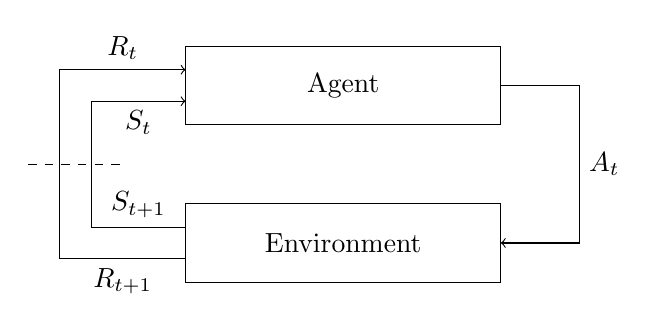
\begin{tikzpicture}
            \draw (0, 2) rectangle node {Agent} (4, 3);
            \draw (0, 0) rectangle node {Environment} (4, 1);

            \draw [->] (4, 2.5) -- (5, 2.5) -- node[right] {$A_t$} (5, 0.5) -- (4, 0.5);

            \draw [->] (0, 0.3) -- node[below] {$R_{t+1}$} (-1.6, 0.3) -- (-1.6, 2.7) --node[above] {$R_t$}  (0, 2.7);
            \draw [->] (0, 0.7) -- node[above] {$S_{t+1}$} (-1.2, 0.7) -- (-1.2, 2.3) -- node[below] {$S_t$} (0, 2.3);

            \draw [dashed] (-2, 1.5) -- (-0.8, 1.5);
        \end{tikzpicture}
        \caption{The agent-environment feedback loop in a Markov Decision Process. \cite{bible}}
        \label{fig:mdp_visualization}
    \end{figure}
\end{frame}

\begin{frame}{Policies and Values}
    \begin{itemize}
        \item Goal of an agent: Maximize \textit{return} (sum of future rewards)
        \item Behavior of an agent to reach the goal is called \textit{policy}
        \item \textit{Value} $v_\pi(s)$ is the expected return when following policy $\pi$ in state $s$
        \item Policies and value functions are usually constructed from neural networks
    \end{itemize}
\end{frame}

\begin{frame}[fragile]{Model-Based Reinforcement Learning}
    \begin{figure}
        \centering
        \begin{tikzpicture}[node distance=0.6]
            \node (St) {$S_t$};

            \node [right = of St, draw, rectangle] (f1) {$f$};
            \node [above = of f1] (At) {$\hat{A}_t$};
            \node [below = of f1] (Rtp1) {$\hat{R}_{t+1}$};

            \node [right = of f1] (Stp1) {$\hat{S}_{t+1}$};

            \onslide<2->{
                \node [right = of Stp1, draw, rectangle] (f2) {$f$};
                \node [above = of f2] (Atp1) {$\hat{A}_{t+1}$};
                \node [below = of f2] (Rtp2) {$\hat{R}_{t+2}$};

                \node [right = of f2] (Stp2) {$\hat{S}_{t+2}$};

                \node [right = of Stp2] (dots) {$\dots$};

                \node [right = of dots, draw, rectangle] (f3) {$f$};
                \node [above = of f3] (Atpnm1) {$\hat{A}_{t+n-1}$};
                \node [below = of f3] (Rtpn) {$\hat{R}_{t+n}$};

                \node [right = of f3] (Stpn) {$\hat{S}_{t+n}$};
            }

            \draw [->] (St) -- (f1);
            \draw [->] (At) -- (f1);
            \draw [->] (f1) -- (Rtp1);
            \draw [->] (f1) -- (Stp1);

            \onslide<2->{
                \draw [->] (Stp1) -- (f2);
                \draw [->] (Atp1) -- (f2);
                \draw [->] (f2) -- (Rtp2);
                \draw [->] (f2) -- (Stp2);

                \draw [->] (Stp2) -- (dots);
                \draw [->] (dots) -- (f3);

                \draw [->] (Atpnm1) -- (f3);
                \draw [->] (f3) -- (Rtpn);
                \draw [->] (f3) -- (Stpn);
            }
        \end{tikzpicture}
        \caption{An environment model $f$ being applied recursively to predict the outcome of a trajectory. \nocite{bible, model}}
        \label{fig:recursive_model}
    \end{figure}
\end{frame}

\begin{frame}{Use Cases of Model-Based RL}
    \begin{figure}
        \centering
        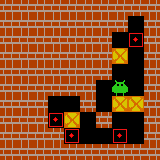
\includegraphics[width=0.5\textwidth]{assets/sokoban.png}
        \caption{Screenshot of the puzzle video game Sokoban. \cite{sokoban}}
        \label{fig:sokoban}
    \end{figure}
\end{frame}

\subsection{MuZero Algorithm}

\begin{frame}[fragile]{MuZero Algorithm}
    \begin{figure}
        \centering
        \begin{tikzpicture}[node distance=0.5]
            \node (ot) {$o_t$};
            \node [left = of ot] (otm1) {$o_{t-1}$};
            \node [right = of ot] (otp1) {$o_{t+1}$};
            \node [left = of otm1] (otm2) {$\dots$};
            \node [right = of otp1] (otp2) {$\dots$};
            \draw [->, dashed] (otm2) -- (otm1);
            \draw [->, dashed] (otm1) -- (ot);
            \draw [->, dashed] (ot) -- (otp1);
            \draw [->, dashed] (otp1) -- (otp2);

            \pause

            \node [below = of ot, draw] (h) {$h_\theta$};
            \node [below = of h] (s0) {$s^0$};
            \draw [->] (ot) -- (h);
            \draw [->] (h) -- (s0);

            \pause

            \node [right = of s0, draw] (g0) {$g_\theta$};
            \node [right = of g0] (s1) {$s^1$};
            \node [above = of g0] (a1) {$a^1$};
            \node [below = of g0] (r1) {$r^1$};
            \draw [->] (s0) -- (g0);
            \draw [->] (a1) -- (g0);
            \draw [->] (g0) -- (s1);
            \draw [->] (g0) -- (r1);

            \node [right = of s1, draw] (g1) {$g_\theta$};
            \node [right = of g1] (s2) {$s^2$};
            \node [above = of g1] (a2) {$a^2$};
            \node [below = of g1] (r2) {$r^2$};
            \draw [->] (s1) -- (g1);
            \draw [->] (a2) -- (g1);
            \draw [->] (g1) -- (s2);
            \draw [->] (g1) -- (r2);

            \node [right = of s2, draw] (g2) {$g_\theta$};
            \node [right = of g2] (s3) {$s^3$};
            \node [above = of g2] (a3) {$a^3$};
            \node [below = of g2] (r3) {$r^3$};
            \draw [->] (s2) -- (g2);
            \draw [->] (a3) -- (g2);
            \draw [->] (g2) -- (s3);
            \draw [->] (g2) -- (r3);

            \pause

            \node [below = of s3, draw] (f) {$f_\theta$};
            \node [below = of f] (pv) {$\policy^3, v^3$};
            \draw [->] (s3) -- (f);
            \draw [->] (f) -- (pv);
        \end{tikzpicture}
        \caption{Testing a single action sequence made up of three actions $a^1$, $a^2$, and $a^3$ to plan based on observation $o_t$ using all three MuZero functions. \nocite{muzero}}
        \label{fig:muzero_basic_policy}
    \end{figure}
\end{frame}

\begin{frame}{MuZero's Loss Function}
    \begin{equation*}
        l_t(\theta) = \sum^K_{k=0} \left(l^r(u_{t+k}, r_t^k) + l^v(z_{t+k}, v_t^k) + l^p(\pi_{t+k}, \policy_t^k) + c||\theta||^2\right)
    \end{equation*}
    \begin{itemize}
        \item Each model output has its own loss term
        \item The model is unrolled through time during training
    \end{itemize}
\end{frame}

\begin{frame}[fragile]{Monte-Carlo Tree Search}
    \begin{figure}
        \centering
        \begin{tikzpicture}
            \node [draw, circle] (s0) {$s^0$};

            \pause

            \node [draw, circle, below left = of s0] (s1) {$s^1$};
            \node [draw, circle, below right = of s0] (s2) {$s^2$};
            \draw [->] (s0) -- node[above left] {$a^1$} (s1);
            \draw [->] (s0) -- node[above right] {$a^2$} (s2);

            \pause

            \node [draw, circle, below left = of s2] (s3) {$s^3$};
            \node [draw, circle, below = of s2] (s4) {$s^4$};
            \node [draw, circle, below right = of s2] (s5) {$s^5$};
            \draw [->] (s2) -- node[above left] {$a^3$} (s3);
            \draw [->] (s2) -- node[right] {$a^4$} (s4);
            \draw [->] (s2) -- node[above right] {$a^5$} (s5);
        \end{tikzpicture}
        \caption{A simplified view of a Monte-Carlo search tree. Note that the number of available actions in state $s^0$ differs from those in state $s^2$. \nocite{mcts}}
        \label{fig:mcts_simple}
    \end{figure}
\end{frame}
